% Space-time grid MILP reference model for relay-drone disaster delivery
% Target version: v5 (26_09_21_03)
% Build: pdflatex milp_en_v5_26_09_21_03.tex
\documentclass[11pt]{article}
\usepackage[margin=1in]{geometry}
\usepackage{amsmath, amssymb, amsthm}
\usepackage{booktabs}
\usepackage{graphicx}
\usepackage{caption}

\newtheorem{proposition}{Proposition}
\DeclareMathOperator*{\argmin}{arg\,min}

\title{A Space--Time Grid MILP Reference Model for\\Relay-Drone Disaster Delivery}
\author{Relay Drone Network project, version v5 (26\_09\_21\_03)}
\date{}

\begin{document}
\maketitle

\begin{abstract}
We give an exact mixed-integer linear programming (MILP) model for the relay-drone
disaster-delivery problem solved by the reinforcement-learning agent and by the geometric
relay heuristic in this project. The model discretises the continuous plane into a regular
lattice augmented with the control centre and the destinations, and discretises time into
periods of $\kappa$ simulator steps chosen so that one period equals exactly one service
time and exactly one lattice move. Relay positions are \emph{not} given in advance: every
lattice node is a candidate. Connectivity to the control centre is imposed in every period
as a single-commodity flow on the graph induced by occupied nodes, which reproduces the
simulator's multi-hop range rule exactly. We state the discretisation conditions under
which the model is feasible, prove the validity of the flow formulation and of the
symmetry-breaking cuts, and validate every solution by replaying it in the simulator.
\end{abstract}

\section{The continuous problem}

A control centre (CC) sits at $p_0 \in \mathbb{R}^2$. A set $D$ of $M$ destinations at
$p_j$, $j \in D$, each requires one parcel. A homogeneous fleet $K$ of $N$ drones starts at
the CC, each loaded with $Q$ parcels. Time advances in simulator steps of $\delta = 1$\,s;
a drone moves at most $v\delta$ per step. Delivering at a destination and reloading at the
CC each freeze the drone for $S$ steps. The mission ends when every destination has
received its parcel; the objective is the makespan.

The defining constraint is communication. Two points can talk if they are within range $R$;
a drone is \emph{connected} if a chain of drones links it to the CC. The simulator enforces
this as a hard constraint at every step: a commanded displacement that would disconnect any
drone is projected back onto the feasible set. Drones are therefore the only relays, and a
drone acting as a relay cannot deliver at the same time. Table~\ref{tab:param} lists the
values used throughout.

\begin{table}[h]
\centering
\caption{Simulator parameters (\texttt{disaster\_relay\_env\_v5\_26\_09\_15\_22}).}
\label{tab:param}
\begin{tabular}{llr}
\toprule
Symbol & Meaning & Value \\
\midrule
$\delta$ & simulator step & $1$\,s \\
$v$ & drone speed & $13.89$\,m/s ($50$\,km/h) \\
$R$ & communication range & $300$\,m \\
$Q$ & parcel capacity & $5$ \\
$S$ & service time (unload at a destination, reload at the CC) & $10$\,steps \\
$\varrho$ & interaction radius for delivery and reload & $25$\,m \\
--- & map & $1000 \times 1000$\,m \\
--- & reachability guarantee of the instance generator & $\|p_j - p_0\| \le 0.9\,N R$ \\
\bottomrule
\end{tabular}
\end{table}

\section{Why the legacy model does not apply}

The model in \texttt{legacy/milp/model.py} was written for an earlier and different problem.
Five of its assumptions conflict with the problem above.

\begin{enumerate}
\item \textbf{One fixed destination per drone.} The map \texttt{k\_dest\_map} assigns drone
$k$ a single destination, so there is no routing decision, no parcel capacity and no reload.
The present problem has $M \gg N$ destinations and capacity $Q < M$.
\item \textbf{Undefined position in transit.} Arcs carry travel times $\tau_{ij} \ge 2$
periods, and the flow balance leaves the drone at no node while it travels. A constraint
that is imposed per period therefore cannot see the drone, so connectivity is enforced only
at the endpoints of a flight that may last many periods.
\item \textbf{Bandwidth instead of range.} Connectivity is modelled as a data flow whose arc
capacities follow a path-loss law $P_0/d^{\alpha}$ with low and high bandwidth demands. The
simulator uses a binary rule: an edge exists if and only if $d \le R$.
\item \textbf{No free relay placement.} The relay set $R$ is empty and the node set consists
of the CC and the destinations, so relays can only hover on top of a destination. In our
problem a relay may need to stop anywhere in the plane.
\item \textbf{Makespan from the service indicator.} $C_k \ge t\,z_{kt}$ measures the last
unloading period of a fixed assignment, not the completion of all $M$ deliveries.
\end{enumerate}

\section{Discretisation}

\paragraph{Time.} Let a period be $\kappa$ simulator steps, $\Delta = \kappa \delta$. We take
$\kappa = S = 10$, so that service occupies exactly one period and the option horizon of the
learned manager ($20$ steps) is exactly two periods. The per-period flight range is
$\ell = v\Delta$.

\paragraph{Space.} Let $G$ be a square lattice of spacing $h$ covering the bounding box of
$\{p_0\} \cup \{p_j\}$ enlarged by $h$, from which we delete nodes farther than $0.9NR$ from
the CC (unreachable, hence useless even as relays) and nodes within $0.35h$ of a point of
interest. The node set is
\[
  N \;=\; \{0\} \;\cup\; D \;\cup\; G ,
\]
so the CC and every destination are exact nodes and the $\varrho$-radius interaction test is
exact. Choosing
\[
  h \;=\; \frac{\ell}{\sqrt{2}}
\]
makes all eight king moves feasible in one period, the diagonal move using the range
exactly. The move set and the communication set are
\[
  A(i) = \{ j \in N : \|p_i - p_j\| \le \ell \} \ni i,
  \qquad
  E = \{ (i,j) \in N^2 : i \ne j,\ \|p_i - p_j\| \le R \} .
\]
Axis-aligned moves cover $h = \ell/\sqrt2$ rather than $\ell$, so the lattice slows a drone
by at most $29\%$ in the axis directions; this is the principal source of discretisation
error and it always acts against the model, never in its favour.

\paragraph{Resolution condition.} The lattice must be fine enough to hold a relay chain.
Serving a destination at distance $d$ from the CC needs at least $\lceil d/R \rceil$ drones,
and the chain has geometric slack $NR - d$. If the lattice cannot place the intermediate
drones to within that slack the instance becomes \emph{infeasible in the model although it is
feasible in the plane}. On the test instance ($N = 3$, $d_{\max} = 791$\,m, slack $109$\,m)
the coarse lattice $h = 196$\,m admits no chain to the farthest destination and the MILP is
infeasible for every horizon, while $h = 98$\,m admits one. A safe rule of thumb is
\[
  h \;\lesssim\; \frac{NR - d_{\max}}{N-1}.
\]

\section{Model}

\subsection{Sets, parameters and variables}

Sets: nodes $N$ with the CC indexed $0$, destinations $D \subset N$, drones $K$,
periods $T = \{0,1,\dots,\bar{T}\}$. Parameters: $Q$, $\ell$, $R$, $A(i)$, $E$, and a
tie-breaking weight $\varepsilon = 10^{-5}$. The horizon $\bar{T}$ is taken from the
heuristic makespan with slack.

\begin{table}[h]
\centering
\caption{Decision variables.}
\begin{tabular}{lll}
\toprule
Variable & Domain & Meaning \\
\midrule
$y_{ikt}$ & $\{0,1\}$ & drone $k$ occupies node $i$ at the boundary of period $t$ \\
$s_{jkt}$ & $\{0,1\}$ & drone $k$ delivers to destination $j$ during period $t$ \\
$r_{kt}$ & $\{0,1\}$ & drone $k$ reloads at the CC during period $t$ \\
$q_{kt}$ & $\{0,\dots,Q\}$ & parcels on board drone $k$ at the boundary of period $t$ \\
$\rho_{kt}$ & $[0,Q]$ & parcels taken on during period $t$ \\
$g_{ijt}$ & $[0,N]$ & connectivity flow on communication arc $(i,j)$ in period $t$ \\
$C$ & $[0,\bar{T}]$ & makespan, in periods \\
\bottomrule
\end{tabular}
\end{table}

\subsection{Objective}

\begin{equation}
\min \; C \;+\; \varepsilon \sum_{i \in N \setminus \{0\}} \sum_{k \in K} \sum_{t \in T} y_{ikt}
\label{eq:obj}
\end{equation}
The second term is a tie-break that prefers plans keeping drones at the CC when this does not
delay the mission; with $\varepsilon \bar{T} N \ll 1$ it cannot change the optimal makespan.

\subsection{Movement and position}

\begin{align}
\sum_{i \in N} y_{ikt} &= 1 && \forall k \in K,\ t \in T \label{eq:one}\\
y_{i,k,t+1} &\le \sum_{j \in A(i)} y_{jkt} && \forall i \in N,\ k \in K,\ t < \bar{T} \label{eq:move}\\
y_{0k0} &= 1 && \forall k \in K \label{eq:start}
\end{align}
Constraint~\eqref{eq:move} states that a drone may occupy $i$ at $t+1$ only if it was at $i$
or at a node from which $i$ is reachable within one period. Because every move takes exactly
one period, the position of every drone is defined at every period boundary --- the property
the legacy model lacks.

\subsection{Deliveries, capacity and reload}

\begin{align}
\sum_{k \in K} \sum_{t < \bar{T}} s_{jkt} &= 1 && \forall j \in D \label{eq:serve}\\
s_{jkt} \le y_{jkt}, \qquad s_{jkt} &\le y_{j,k,t+1} && \forall j \in D,\ k,\ t \label{eq:sat}\\
r_{kt} \le y_{0kt}, \qquad r_{kt} &\le y_{0,k,t+1} && \forall k,\ t \label{eq:rat}\\
\sum_{j \in D} s_{jkt} + r_{kt} &\le 1 && \forall k,\ t \label{eq:busy}\\
\sum_{j \in D} s_{jkt} &\le q_{kt} && \forall k,\ t \label{eq:cap}\\
q_{k,t+1} &= q_{kt} - \sum_{j \in D} s_{jkt} + \rho_{kt} && \forall k,\ t \label{eq:bal}\\
\rho_{kt} \le Q\, r_{kt}, \qquad q_{k,t+1} &\ge Q\, r_{kt} && \forall k,\ t \label{eq:full}\\
q_{k0} &= Q && \forall k \label{eq:load0}
\end{align}
The pair in~\eqref{eq:sat} encodes the service freeze: the drone must be at the destination
when it delivers and must still be there one period later, which is exactly the $S = \kappa$
steps during which the simulator blocks its motion. Constraints~\eqref{eq:full} together with
$q \le Q$ force a reload to fill the drone completely, as the simulator does.

\subsection{Connectivity}

Write $u_{it} = \sum_{k \in K} y_{ikt}$ for the occupancy of node $i$ and set $u_{0t} := 1$.
Every occupied node ships one unit of flow to the CC, which is the only sink:
\begin{align}
\sum_{j : (i,j) \in E} g_{ijt} \;-\; \sum_{j : (j,i) \in E} g_{jit} &= u_{it}
   && \forall i \in N \setminus \{0\},\ t \in T \label{eq:flow}\\
g_{ijt} &\le N\, u_{it} && \forall (i,j) \in E,\ t \in T \label{eq:cap2}
\end{align}

\begin{proposition}[Correctness]
For a fixed occupancy $u_{\cdot t}$, the system \eqref{eq:flow}--\eqref{eq:cap2} is feasible
if and only if every occupied node is joined to node $0$ by a path whose intermediate nodes
are occupied and whose consecutive distances are at most $R$; that is, if and only if the
simulator's multi-hop connectivity test succeeds.
\end{proposition}

\begin{proof}
($\Leftarrow$) Send one unit from each occupied node along such a path; \eqref{eq:cap2} holds
because every arc used leaves an occupied node, and at most $N$ units traverse any arc.
($\Rightarrow$) Let $i \ne 0$ be unoccupied. Then \eqref{eq:cap2} forces $g_{ijt} = 0$ for all
$j$, and \eqref{eq:flow} gives $\sum_j g_{jit} = 0$, so no flow passes through $i$. Hence all
flow travels inside the occupied set. Node $0$ is the only node without a conservation
constraint, so the $\sum_i u_{it}$ units supplied must be absorbed there, and a flow
decomposition yields a path from every occupied node to $0$.
\end{proof}

\begin{proposition}[Redundancy of the head capacity]
Adding $g_{ijt} \le N u_{jt}$ for $j \ne 0$ does not change the feasible set.
\end{proposition}

\begin{proof}
Immediate from the second half of the previous proof: an unoccupied node carries no flow at
all, so no arc entering it can be positive.
\end{proof}

This halves the number of capacity rows, which dominate the model size
($|E|\,|T|$ rows rather than $2|E|\,|T|$).

\subsection{Makespan and symmetry}

\begin{align}
C &\ge t\, s_{jkt} && \forall j \in D,\ k \in K,\ t < \bar{T} \label{eq:mk}\\
s_{jkt} &= 0 && \forall k \in K,\ j \in D \text{ with } \mathrm{idx}(j) < k+1,\ t < \bar{T} \label{eq:sym}
\end{align}

\begin{proposition}[Validity of \eqref{eq:sym}]
The cut removes no solution value. 
\end{proposition}

\begin{proof}
Drones are identical, so any solution may be relabelled. Order the drones by the smallest
index of a destination they serve, placing drones that serve none last. Under this labelling
the smallest index served by drone $k$ (1-based) is at least $k$, because the minima are
distinct and increasing. Hence drone $k$ serves no destination of index below $k$.
\end{proof}

\section{What the optimum means}

Two effects separate the model from the continuous problem, and both must be stated.

\paragraph{Restriction.} Drones are confined to lattice nodes and to period boundaries, and
axis moves waste up to $29\%$ of the range. Every grid plan maps to a physically flyable
trajectory (each move is a straight segment of length at most $\ell$ flown within $\Delta$),
so the model explores a strict subset of the continuous plans. Its optimum is therefore an
\emph{upper} bound on the continuous optimum, not a certificate of optimality.

\paragraph{Sampling of the connectivity constraint.} The model imposes connectivity at period
boundaries. Between two boundaries the drones fly simultaneously and the chain may break
transiently. We therefore do not claim feasibility: we \emph{verify} it, by replaying the
plan in the simulator with the same straight-line low-level controller used by all other
methods and counting the steps in which the simulator's projection had to cut a commanded
displacement. As $\kappa \to 1$ the sampling becomes the simulator's own test and the effect
vanishes; the price is $|T| \propto \kappa^{-1}$.

\paragraph{Lower bound.} A valid lower bound on the continuous optimum is
\[
  C_{\mathrm{LB}} \;=\; \max\!\left\{ \frac{d_{\max}}{v},\ \left\lceil \frac{M}{N} \right\rceil S \right\},
\]
the flight time to the farthest destination and the service time that $N$ parallel servers
need for $M$ deliveries. Together with the model optimum it brackets the true optimum.

\section{Computational study}

The instances come from the project's own generator (\texttt{sample\_instance}, seed 901) with $N = 3$ drones, so that the MILP, the heuristic and the learned policy all see the same geometry. Gurobi 13.0.2 ran with six threads on a machine that was concurrently training the reinforcement-learning agent. The lattice uses $\kappa = 10$ simulator steps per period and $h = 98.2$\,m.

\begin{table}[h]
\centering
\caption{Model size and search outcome. Makespan is in simulator steps (seconds). ``best'' is the best incumbent over the runs listed; the spread shows how much the incumbent varies between identical runs with different solver seeds.}
\label{tab:milp}
\begin{tabular}{rrrrrrrr}
\toprule
$M$ & $|N|$ & $\bar{T}$ & binaries & runs & best & spread & bound \\
\midrule
4 & 99 & 18 & 5913 & 5/5 & 140 & 140--170 & 81 \\
6 & 98 & 23 & 7539 & 1/2 & 180 & --- & 100 \\
10 & 107 & 30 & 10941 & 0/2 & none & --- & --- \\
\bottomrule
\end{tabular}
\end{table}

\begin{table}[h]
\centering
\caption{The best MILP plan replayed in the simulator, against the geometric relay rule with deadlock escape on the same instance. ``cut'' counts the drone-steps in which the simulator's connectivity projection shortened a commanded displacement, the price of sampling connectivity only at period boundaries.}
\label{tab:replay}
\begin{tabular}{rrrrrr}
\toprule
$M$ & MILP & replayed & cut steps & rule & $C_{\mathrm{LB}}$ \\
\midrule
4 & 140 & 138 & 22 & 145 & 50 \\
6 & 180 & 176 & 59 & 185 & 53 \\
10 & none & --- & --- & 244 & 57 \\
\bottomrule
\end{tabular}
\end{table}

Two facts stand out. The incumbent is unstable: 5 runs of the same $M = 4$ model with different solver seeds returned makespans from 140 to 170\,s. And the primal side degrades sharply with the number of destinations: at $M = 4$, 5 of 5 runs returned a feasible plan, at $M = 6$, 1 of 2 runs returned a feasible plan, at $M = 10$, 0 of 2 runs returned a feasible plan. The model is a reference for the smallest instances only. Where it does return a plan, the plan is good: replayed in the simulator it beats the geometric rule with deadlock escape (138 against 145\,s at $M = 4$; 176 against 185\,s at $M = 6$), and it never loses connectivity. The cut-step counts in Table~\ref{tab:replay} are the price of sampling connectivity at period boundaries: the simulator had to shorten that many commanded displacements, without ever disconnecting a drone.

\begin{figure}[h]
\centering
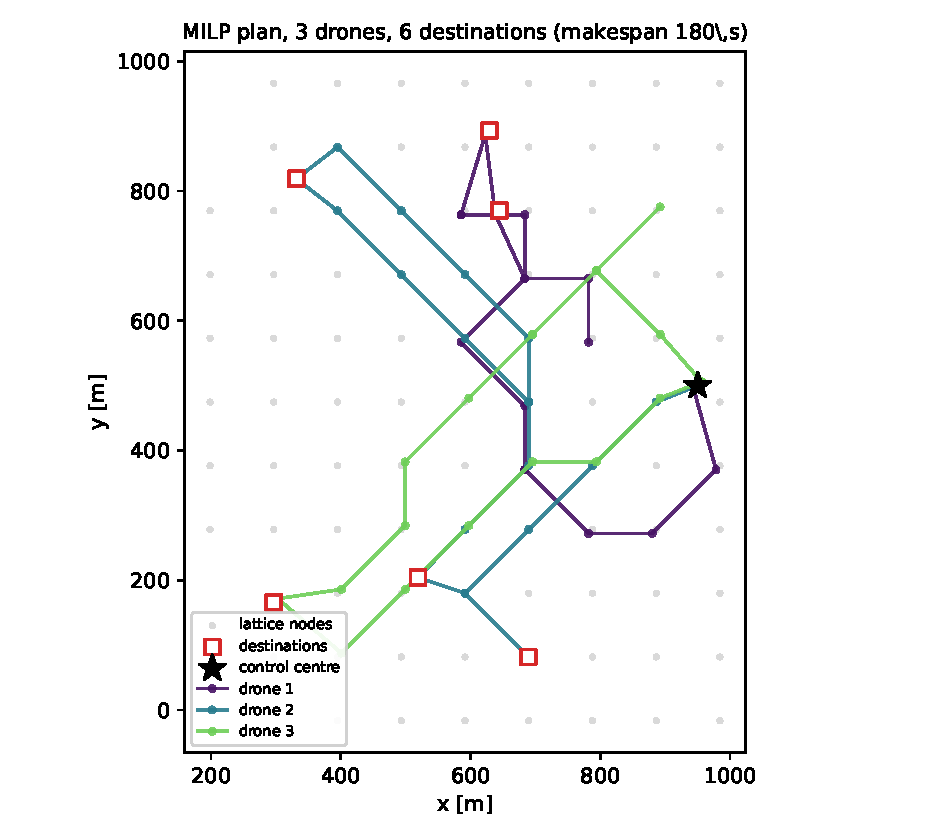
\includegraphics[width=0.70\textwidth]{../../figures/milp_plan_v5_26_09_21_03.pdf}
\caption{Lattice, destinations and optimal trajectories for the largest instance the model could solve. Trajectories are offset by a few metres per drone so that shared nodes stay visible.}
\label{fig:plan}
\end{figure}


\section{Limitations}

The model scales as $|N|\,|K|\,|T|$ binaries and $|E|\,|T|$ continuous variables, with
$|N| = \Theta(h^{-2})$ and $|T| = \Theta(\kappa^{-1})$, and the resolution condition ties $h$
to the chain slack. Instances with many drones or destinations are out of reach; the model is
a reference point for small instances, not a solution method. It also inherits the two
approximations of the previous section, and it assumes, as the simulator does, that service
times are deterministic and that no drone fails.

\end{document}
